\subsubsection{Direct Linking (\texttt{-L})}
\label{section:direct-linking}

As described in \autoref{section:jit-arch}, each compiled host block terminates by returning the target MIPS address; this implementation is required for supporting branching as the desired MIPS address may not yet have a corresponding compiled x86 block. By first returning to the runtime the desired block can first be compiled if necessary.

While this provides flexibility, it does lead to non-ideal performance once the necessary blocks have been compiled. \autoref{figure:jit-steady} illustrates the execution flow of the JIT emulator when all the relevant blocks have been compiled. In some cases, such as loops in the source code, this leads to an undesirably large overhead in the emulation. This is because for every iteration of the loop, the control flow must return from the compiled x86 block to the runtime which checks if the destination block has been compiled then returns control flow back to the compiled x86 block; while these dispatch overheads seem trivial, profiling has shown that they can become significant bottlenecks for hot loops.

The direct linking feature, denoted by \texttt{-L}, was developed to remedy this. It is available for both the JIT and hybrid emulators. Direct linking allows the emulator to retroactively patch the end of the block to have a native jump to its target x86 block instead of returning to the runtime. This allows the emulated program to eventually become a native x86 program that does not require the runtime for dispatching, but is still able to use the runtime to compile and dispatch to unseen blocks.

\begin{figure}[h]
    \centering
    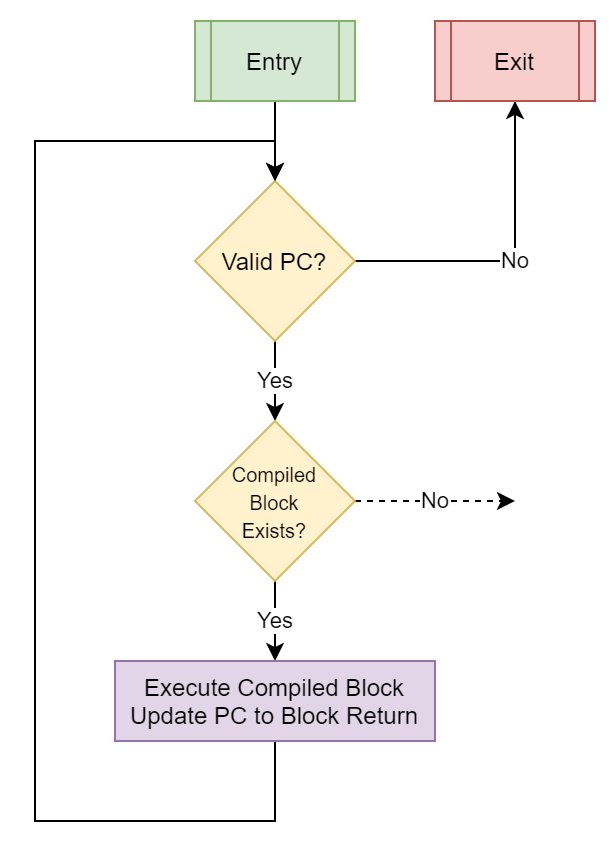
\includegraphics[width=0.5\linewidth]{diagrams/jit-steady.png}
    \caption{The execution flow of the JIT emulator when all source blocks have been translated.}
    \label{figure:jit-steady}
\end{figure}

In order to support direct linking, all unresolved jumps must be stored for each x86 block compiled; the x86 address of the terminal is stored so that it can be patched with a direct jump, and the desired MIPS target address is stored so that the corresponding x86 block can be found. When a new x86 block is compiled, all existing x86 blocks will be tested for relinking; if any unresolved jumps are found with a target MIPS address that now has an entry in the translation table, the terminal will be overwritten with a direct jump to the corresponding x86 block.

This should allow for much higher execution performance at the cost of additional overheads as extra work needs to be performed to track the unresolved jumps and perform the relinking. On the surface, it may appear that relinking every block when a new block is compiled is wasteful; we have to check more blocks for relinking and may perform relinking on a block that is never executed again. It might then be reasonable to assume that instead the runtime should only relink the block that is about to be executed: \autoref{figure:relinking} illustrates a scenario which demonstrates why this is not the case.

In the following scenario, when only relinking the current block, \texttt{block\_1} is directly linked to \texttt{block\_2} when \texttt{block\_1} is executed. Executing \texttt{block\_1} now causes a direct jump to \texttt{block\_2}, which then terminates and uses the runtime to dispatch to \texttt{block\_3}. In this case, \texttt{block\_2} can no longer be executed directly from the runtime and is only ever executed as a direct jump from \texttt{block\_1}; this means that the runtime never performs relinking on \texttt{block\_2}, stopping \texttt{block\_2} from directly jumping to \texttt{block\_3}. This is not ideal as it greatly reduces the peak performance of the emulated program.

\begin{figure}[h]
    \centering
    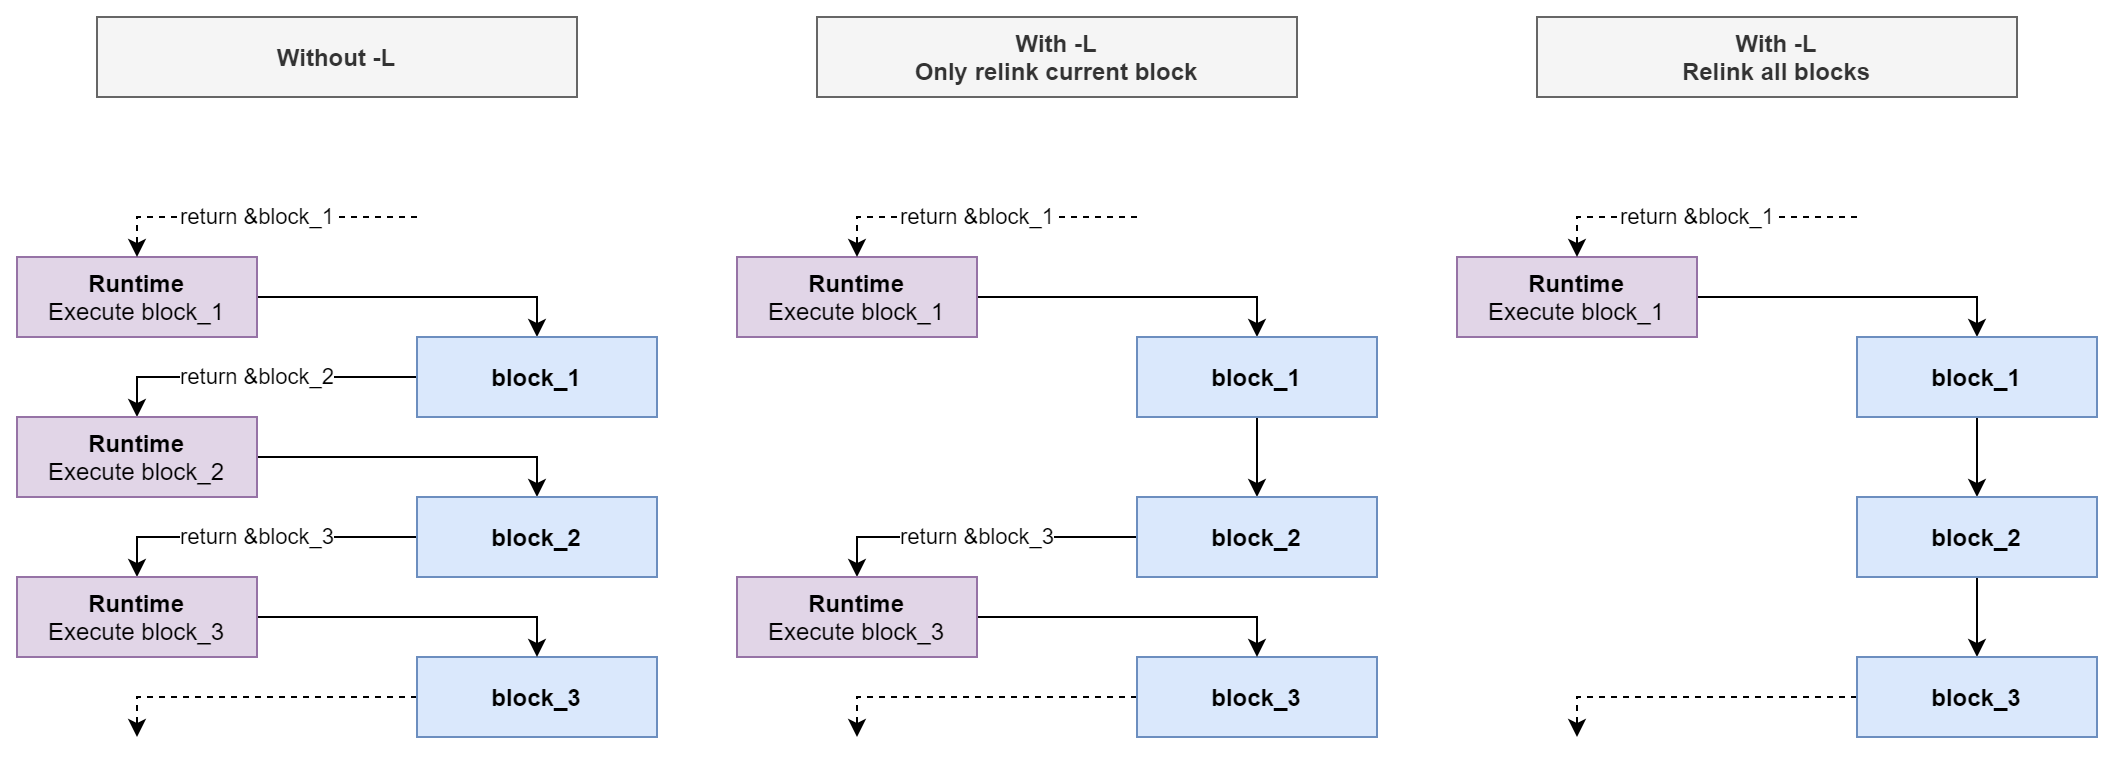
\includegraphics[width=1\linewidth]{diagrams/relinking.png}
    \caption{The effects of different relinking schemes on an example program fragment consisting of 3 blocks.}
    \label{figure:relinking}
\end{figure}

Unconditional jumps, such as \texttt{J} and \texttt{JAL} are the simplest to relink. They contain a single target MIPS address and a single x86 source address. If the MIPS target is present in the translation table, then the source x86 address (pointing to the current terminal) will be overwritten with a jump to the x86 block corresponding to the target MIPS address.

Conditional jumps, on the other hand, have two target MIPS addresses. This is because conditional jumps are implemented by having a \textit{true} jump to the desired address in the MIPS source code and a \textit{false} jump to the following instruction. Due to this a simple implementation would require that both targets are present in the translation table before relinking can proceed.

\begin{lstfloat}[h]
    \begin{lstlisting}
init:
    addi $1, $0, 0
    addi $2, $0, 0

loop_start:
    add  $2, $2, $1
    addi $1, $1, -1
    bne  $1, $0, loop_start
    nop

loop_end:
    add  $1, $2, $0

    \end{lstlisting}
    \caption{An example MIPS program containing a simple loop.}
    \label{code:relinking-loop}
\end{lstfloat}

\autoref{code:relinking-loop} details an example MIPS program with a typical loop, with the \texttt{BNE} on line \texttt{8} being the branch of interest. After the first iteration of the loop, the \textit{true} case jumps to \texttt{loop\_start} which has a corresponding x86 block compiled, yet the \textit{false} case jumps to \texttt{loop\_end}, which does not yet have a corresponding x86 block; in fact, \texttt{loop\_end} would not be translated until the loop has finished execution. This means the branch cannot be relinked until the loop has terminated, somewhat defeating the purpose of relinking.

By performing partial relinking this can be remedied. For conditional branches, if either the \textit{true} or \textit{false} cases are present in the translation table, then that half of the branch can be relinked whilst the other case is left as a dispatch to the runtime. A partially relinked branch can then be fully relinked and resolved later once both destinations are present in the translation table.

The instructions \texttt{JR} and \texttt{JALR} cannot be relinked; this is because their target MIPS address is determined by the contents of a register, and thus the desired target of the jump cannot be known at (JIT) compile time. The MIPS address must be resolved to a corresponding x86 block dynamically by dispatching to the runtime. In practice, this means function returns cannot be relinked.